\section{Model IV: Temporal Dynamics}\label{sec:model-temporal}

\subsection{Revolutions as Punctuated Leaps (Task~5)}\label{subsec:t5-revolutions}

Task~5 asks which characteristics mark \emph{revolutions} (major leaps) in
musical evolution, and which artists are the corresponding revolutionaries.
We treat change as \emph{punctuated cultural evolution}: variants in a
population drift continuously~\cite{savage2019cultural}, but the rate of
change can spike in short windows~\cite{mauch2015evolution}. Operationally:

\begin{itemize}[leftmargin=1.2em,itemsep=0.2em]
  \item \textbf{Evolution:} gradual movement of the yearly feature state and
  slow change of cross-genre influence shares.
  \item \textbf{Revolution:} a short window in which the sonic leap size is
  anomalous relative to its recent baseline, optionally reinforced by a
  simultaneous restructuring of the influence network.
\end{itemize}

\paragraph{Sonic channel.}
Let \(\mathbf{x}(t)\in\mathbb{R}^{p}\) be the vector of the same \(p=11\)
Spotify features as Model~II, taken from \texttt{data\_by\_year} and
\(z\)-scored across years \(t\in[1930,2010]\). The sonic leap size is
\begin{equation}\label{eq:t5-E}
E(t)=\|\mathbf{x}(t)-\mathbf{x}(t-1)\|_2.
\end{equation}
Because early catalogue aggregates are thin and inflate a global threshold,
we score each \(E(t)\) by a rolling \(z\)-score against the preceding
12 leaps and call a \emph{sonic anomaly} when this local \(z\geq 2\) and
\(t\geq 1948\). The coordinates of \(\Delta\mathbf{x}(t)\) with largest
absolute share identify the driving characteristics of each leap. A Foote-style
past/future window novelty is retained as a robustness companion (same
qualitative peaks).

\paragraph{Network channel.}
We reuse the teammate Model~III flow layer without redefining it: \(F(t)\)
is the genre-to-genre edge count matrix restricted to followers whose
active-start decade is \(t\), with cross-genre share \(c_{\mathrm{cross}}(t)\)
and Katz-weighted share \(c_K(t)\). Decade restructuring is summarised by
\begin{equation}\label{eq:t5-N}
N(t)
=\tfrac12\bigl|\Delta c_{\mathrm{cross}}(t)\bigr|
+\tfrac12\bigl|\Delta c_K(t)\bigr|
+\tfrac14\,\tau(t),
\end{equation}
where \(\tau(t)\) is the \(\ell_1\) turnover of genre shares of outgoing
Katz mass \(K_g(t)\) among artists starting in decade \(t\). Decades with
\(z\)-scored \(N(t)\) above \(0.75\) are network anomalies. This keeps the
same follower-start decade clock as Assumption~A2 and as \(F(t)\), \(c_K(t)\)
in \cref{subsec:q3-inf-time}.

\paragraph{Dual-channel labels.}
A decade is \emph{strong} if it contains at least one sonic anomaly and is a
network anomaly; \emph{weak} if exactly one channel fires; otherwise
\emph{evolution}. Empirically the only strong decade is the 1970s (sonic
peak in 1976; sharp drop in \(c_{\mathrm{cross}}\) and \(c_K\) after the
1950--60s cross-genre high). The 1950s are a network-only weak signal:
\(c_K(t)\) peaks near \(0.53\) while local sonic \(z\) stays below the
cutoff---an influence-structure rewiring (rock \& roll / R\&B export) that
is louder in \(F(t)\) than in yearly mean features. Pre-1948 spikes in raw
\(E(t)\) are plotted but not labelled revolutions (composition caution).

\begin{figure}[t]
\centering
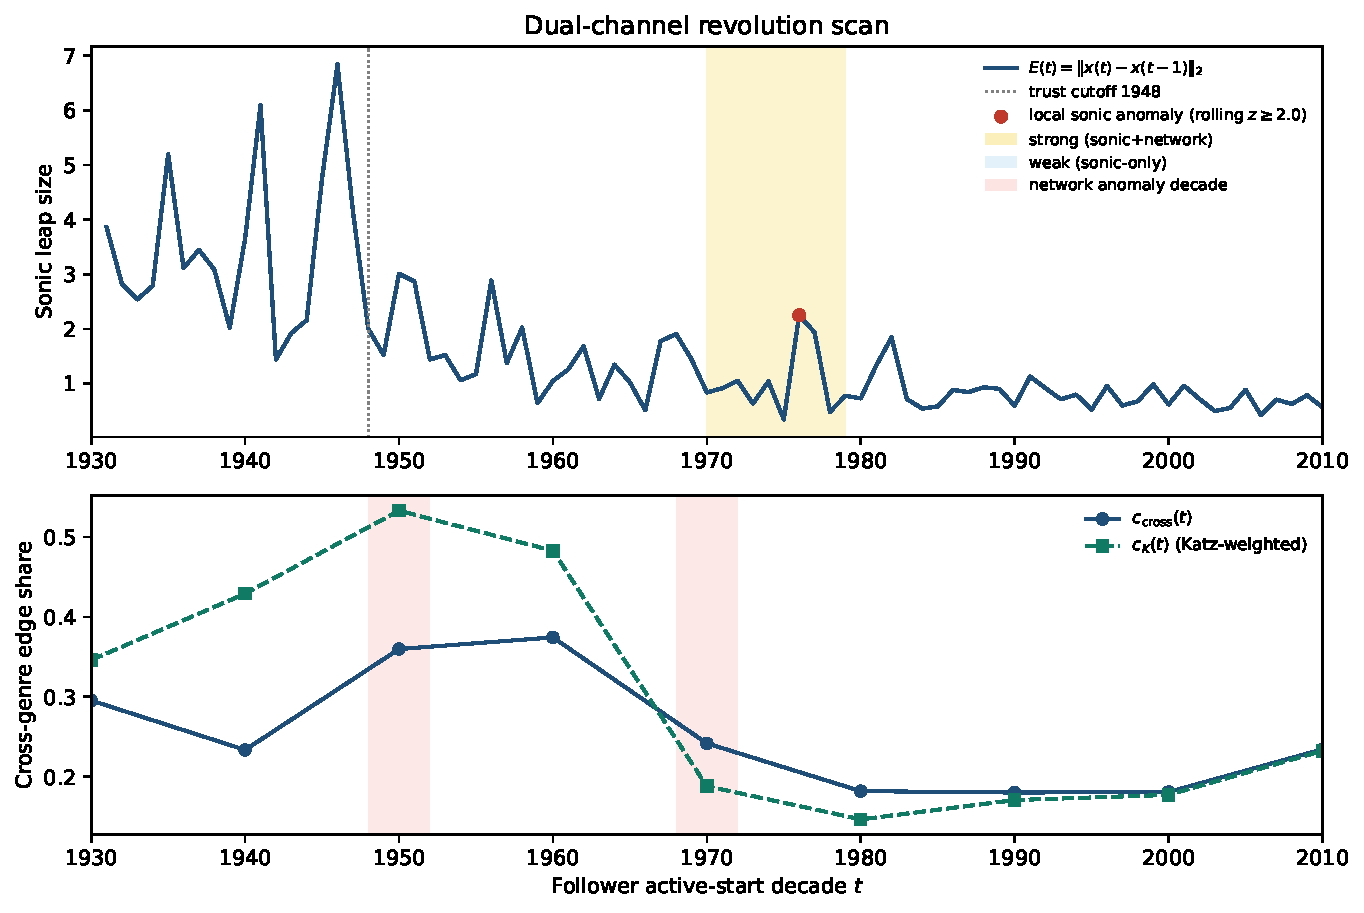
\includegraphics[width=0.68\textwidth]{fig_t5_dual_channel_revolutions.pdf}
\caption{Dual-channel scan: sonic leap \(E(t)\) (top; local \(z\geq 2\),
\(t\geq 1948\)) and network shares \(c_{\mathrm{cross}}(t)\), \(c_K(t)\)
(bottom). Gold = strong 1970s; network-only weak = 1950s.}
\label{fig:t5-dual}
\end{figure}

\paragraph{Characteristics that signify leaps.}
In the strong 1970s window the dominant driver of \(\Delta\mathbf{x}\) is
\texttt{liveness}, followed by \texttt{duration\_ms} and \texttt{tempo}:
the leap is a production/performance shift rather than a single
``genre birth'' coordinate. Network-side, the signifying quantity is the
collapse of cross-genre share after its mid-century plateau
(\(c_{\mathrm{cross}}\approx 0.36\)--\(0.37\) in 1950--60 down to
\(\approx 0.18\) by 1980--2000), i.e.\ influence re-concentrates inside
genres even while sonic drift continues slowly.

\paragraph{Revolutionaries.}
Within a flagged decade \(d\) we score artists who began no later than \(d\)
by a blend of outgoing Katz \(K_i\), the number of followers whose
active-start lies in \(\{d,d+10\}\), and the alignment of their feature
displacement from the previous-decade mean of \(\mathbf{x}(t)\) with the
window's mean sonic direction \(\Delta\mathbf{x}\). This prefers transmitters
who move \emph{with} the leap and are followed afterward, not artists who
merely correlate with the industry average. Top names in the 1950s weak
window include Chuck Berry, Little Richard and James Brown; in the 1970s
strong window, Bob Dylan, The Rolling Stones and Jimi Hendrix
(\cref{tab:t5-revs}).

\begin{table}[htbp]
\centering
\caption{Top revolutionaries by dual-channel window (score blend of \(K_i\),
followers in \(\{d,d+10\}\), and sonic alignment).}
\label{tab:t5-revs}
\small
\begin{tabular}{cllll}
\toprule
Decade & Label & Artist & Genre & \(K_i\) rank signal \\
\midrule
1950s & weak (network) & Chuck Berry & Pop/Rock & high \(K_i\), many 1950/60 followers \\
1950s & weak (network) & Little Richard & Pop/Rock & high alignment + followers \\
1950s & weak (network) & James Brown & R\&B & cross-genre transmitter \\
1970s & strong & Bob Dylan & Pop/Rock & top score in window \\
1970s & strong & The Rolling Stones & Pop/Rock & high \(K_i\) + followers \\
1970s & strong & Jimi Hendrix & Pop/Rock & strong sonic alignment \\
\bottomrule
\end{tabular}
\end{table}

\paragraph{Limits.}
\texttt{data\_by\_year} is a Spotify-era mean catalogue, not a probability
sample of all music; early \(E(t)\) is composition-sensitive. Influence edges
are reported relations, and decade \(t\) indexes follower start years, not
event dates. Detected leaps are statistical rate spikes, offered as
candidates for historical interpretation rather than causal claims.

% T6 is included from main.tex via model4_t6.tex (after this Model IV / Task~5 block).
% TODO (T7): pre/post-1995 era slicing; internet effect on network + features.
